\newpage
\section{Gestione questionari}
Selezionata la voce \textit{Gestione questionari} dal menù a sinistra il sistema visualizza la seguente pagina, dalla quale un utente può gestire i propri questionari:

\label{GestioneQuestionari}
\begin{figure}[ht]
	\centering
	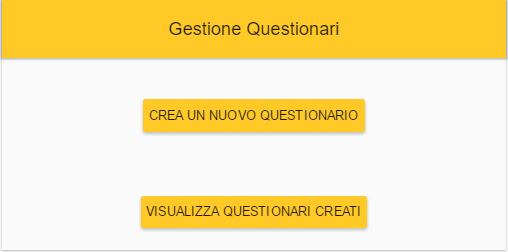
\includegraphics[scale=0.55]{img/gestione_questionari.png}
	\caption{Gestione questionari}
\end{figure}
\FloatBarrier

\newpage
\subsection{Crea un nuovo questionario}
Selezionando la voce \textit{CREA UN NUOVO QUESTIONARIO} si avvia la funzionalità di creazione di un questionario:

\label{CreazioneQuestionari}
\begin{figure}[ht]
	\centering
	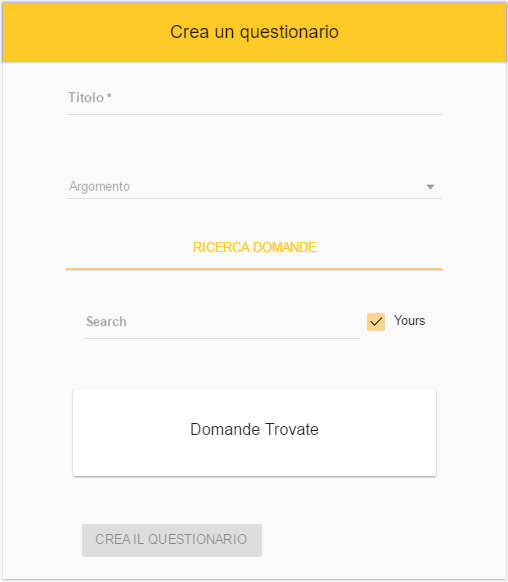
\includegraphics[scale=0.55]{img/creazione_questionario.png}
	\caption{Creazione questionario}
\end{figure}
\FloatBarrier

Sara possibile scegliere un \textit{Titolo} e un \textit{Argomento} da associare al questionario che si sta creando. In più si potranno inserire le domande ricercandole tra le proprie create oppure all'interno del sistema, digitando le parole chiave associate. Compilati tutti i campi dati necessari il bottone \textit{CREA IL QUESTIONARIO} viene abilitato e permetterà di creare il questionario. 

\newpage
\subsection{Gestione questionari creati}
Dopo il pulsante di creazione questionari, la pagina mostra un elenco di tutti i questionari creati dall'utente. Per ogni questionario è possibile:
\begin{itemize}
	\item Gestire le iscrizioni;
	\item Abilitarlo alla compilazione.
\end{itemize}

\label{GestioneQuestionario}
\begin{figure}[ht]
	\centering
	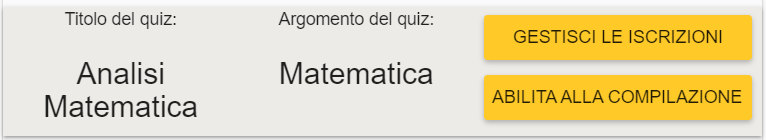
\includegraphics[scale=0.55]{img/gestione_questionario.png}
	\caption{Gestione questionario}
\end{figure}
\FloatBarrier

Nella sezione \textit{GESTISCI LE ISCRIZIONI}, l'utente può visualizzare tutti gli utenti iscritti al questionario e decidere, per ognuno, se abilitarli alla compilazione o meno. Cliccando infine sul bottone \textit{ABILITA ALLA COMPILAZIONE}, ogni utente precedentemente abilitato può ora compilare il questionario. 
